%! Suppress = MissingImport
\section{Abstract workflow}\label{sec:abstract-workflow}

This section will present the new proposed abstract workflow and highlight
the new steps and main points.

\begin{figure}
    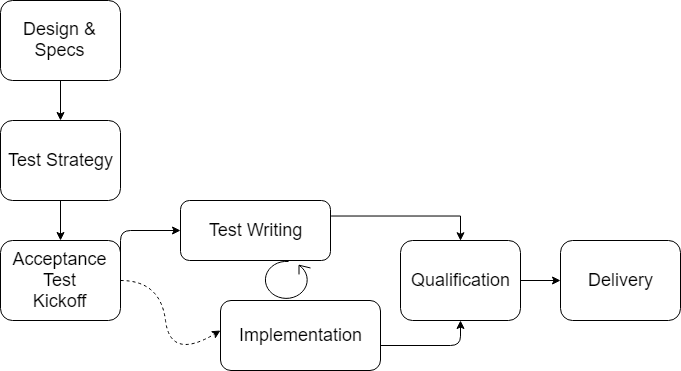
\includegraphics[width=\textwidth]{../../resources/images/solution/new_workflow.png}
    \centering
\end{figure}

\subsubsection{Traditional beginning and ending}
The beginning and ending of this new workflow aren't really new, they're both
inherited from the traditional waterfall / V-model methodologies.
From a black box perspective, the process haven't really changed, the client
will still have the documentation, qualification reports and a delivery at
the end.

\subsubsection{Acceptance Test Kickoff}
This phase is the main new one and extends the Test Strategy phase.
Since the solution is going to use the approach of Acceptance Test Driven
Development, the test writing phase must be well prepared before starting it.

This new phase has been specifically made to structure the scenario format,
domain vocabulary etc.
to build a reliable base for the following steps.

Note that this phase is only relevant at the first iteration of the project.
Once the setup is done and validated, further iterations will be able to skip
it and will therefore be lighter and quicker.

\subsubsection{Parallel Test \& Implementation}
In this new workflow, the test writing and implementation phases are now
running in parallel but don't start at the same time.
After the Acceptance Test Kickoff, the test writing phase starts first.
The testers use the base built during the kickoff and start producing new
scenarios in the backlog.
Once the backlog contains enough features, the implementation phase can start.

The implementation is slightly delayed to ensure that the features are not
developed to quickly.
This would force the developers to wait for the testers to write new
scenarios and also encourage the testers to write the features in rush, which
would increase the risk of error.

There is a continuous communication and feedback between the developers and
testers regarding the scenarios.
They are at the core of the process so they must be made and maintained by
the both team.
